\documentclass[11pt]{article}

\usepackage[margin=1in]{geometry}
\usepackage{graphicx}
\usepackage{booktabs}
\usepackage{amsmath}
\usepackage{hyperref}
\usepackage{xcolor}
\usepackage{listings}
\usepackage{caption}
\usepackage{float}
\usepackage{enumitem}
\usepackage{fancyhdr}
\usepackage{titlesec}
\setlength{\headheight}{14pt}

\hypersetup{
    colorlinks=true,
    linkcolor=blue,
    urlcolor=blue,
    citecolor=blue
}

\titleformat{\section}{\large\bfseries}{\thesection}{1em}{}
\titleformat{\subsection}{\normalsize\bfseries}{\thesubsection}{1em}{}

\pagestyle{fancy}
\fancyhf{}
\rhead{Credit Risk Decision System}
\lhead{Technical Report}
\rfoot{\thepage}

\title{\textbf{A Production-Grade Credit Risk Decision System:\\
From Exploratory Analysis to Deployed ML Service}}
\author{Saumi \\ \small \href{https://github.com/Saumi18/Credit-Risk-Modeling}{github.com/Saumi18/Credit-Risk-Modeling} \\ \small \href{https://credit-risk-modeling.vercel.app}{Live Demo}}
\date{\today}

\begin{document}

\maketitle

\begin{abstract}
This report documents the design, implementation, and deployment of a full-stack
credit risk decision system that predicts the probability of credit card default.
The system was built incrementally: data cleaning and leakage-safe feature
engineering, imbalanced-classification modeling with honest evaluation metrics,
hyperparameter and decision-threshold optimization, SHAP-based explainability,
and a production-style engineering layer consisting of a FastAPI backend,
PostgreSQL persistence, Redis caching, asynchronous batch processing via a
job queue, full Docker containerization, and live cloud deployment. The final
tuned LightGBM model achieves an F1 score of 0.545 and an AUC of 0.778 on a
held-out test set, evaluated on the UCI Default of Credit Card Clients dataset
(30{,}000 applicants, 22.1\% positive class). This report also documents
several concrete engineering decisions and trade-offs made along the way --
including a rejected SMOTE experiment, a cross-platform worker bug, and a
free-tier deployment constraint -- as evidence of an iterative, evidence-based
engineering process rather than a one-shot script.
\end{abstract}

\tableofcontents
\newpage

% ============================================================
\section{Introduction}
% ============================================================

Credit risk modeling -- estimating the probability that a borrower will
default on an obligation -- is one of the most consequential applications
of applied machine learning, directly informing lending decisions that
affect real people's access to credit. This project builds a complete,
deployable system around this problem, treating it not purely as a modeling
exercise but as a full software engineering task: the trained model is one
component embedded inside a backend service, a database layer, an
asynchronous processing pipeline, and a live web application.

\subsection{Objectives}
\begin{itemize}[nosep]
    \item Build a leakage-free, reproducible modeling pipeline on a real,
    publicly available, imbalanced dataset.
    \item Evaluate the model honestly using metrics appropriate for class
    imbalance (precision, recall, F1, AUC), not raw accuracy.
    \item Make and document real engineering trade-offs (e.g., SMOTE vs.
    class weighting, thread vs. process-based background workers) backed
    by measurement rather than assumption.
    \item Package the model behind a production-style API with persistence,
    caching, and asynchronous batch processing.
    \item Deploy the complete system to the public internet with a
    user-facing interface.
\end{itemize}

\subsection{Scope and honest limitations}
This is a portfolio and demonstration project. The model is trained on a
single historical dataset from Taiwanese credit card customers (2005) and
is explicitly \textbf{not} calibrated for real-world lending decisions in
any other population or time period. Where results might otherwise appear
impressive, this report favors transparency over inflated claims -- for
example, this dataset is a recognized difficult benchmark, and published
results in the literature typically fall in the 0.75--0.82 AUC range, not
higher; this system's results are consistent with that range and are
reported as such.

% ============================================================
\section{Dataset}
% ============================================================

The \textbf{UCI Default of Credit Card Clients} dataset~\cite{uci_dataset}
was used, comprising 30{,}000 credit card holders in Taiwan, with 23
original features and a binary target (default in the following month:
yes/no).

\subsection{Class balance}
The target variable is imbalanced: 77.9\% of applicants did not default,
and 22.1\% did. This imbalance is central to every subsequent modeling
decision in this report -- a naive classifier that always predicts ``no
default'' would already achieve 77.9\% accuracy while being entirely
useless, which is why accuracy is deliberately not used as a headline
metric anywhere in this work.

\subsection{Data quality issues identified}
Exploratory analysis surfaced two data-quality issues that required
explicit handling:
\begin{itemize}[nosep]
    \item \textbf{Undocumented category codes}: the \texttt{EDUCATION}
    field contains categories 0, 5, and 6 that are not defined in the
    dataset's documentation (which only defines 1--4). Similarly,
    \texttt{MARRIAGE} contains an undocumented category 0. Rather than
    dropping these rows (which would non-randomly remove data, since these
    codes are not missing-at-random), they were collapsed into an explicit
    ``other/unknown'' bucket.
    \item \textbf{Naming inconsistency}: the repayment status column for
    the most recent month is named \texttt{PAY\_0} in the raw data, while
    subsequent months are \texttt{PAY\_2} through \texttt{PAY\_6} --
    skipping \texttt{PAY\_1}. This was corrected by renaming
    \texttt{PAY\_0} to \texttt{PAY\_1} for consistency throughout the
    pipeline.
\end{itemize}

% ============================================================
\section{Methodology}
% ============================================================

\subsection{Feature engineering}
Beyond the 23 raw features, seven additional features were engineered
from within-row arithmetic (i.e., no aggregation across rows, which would
risk leakage if computed before the train/test split):

\begin{itemize}[nosep]
    \item \texttt{avg\_bill\_amt}, \texttt{avg\_pay\_amt}: mean bill and
    payment amounts across the 6 observed months.
    \item \texttt{utilization\_ratio}: average bill amount relative to
    credit limit -- a standard credit risk signal.
    \item \texttt{payment\_ratio}: average payment amount relative to
    average bill amount, capturing repayment behavior.
    \item \texttt{delay\_trend}: difference between the most recent and
    oldest repayment status, capturing whether behavior is improving or
    deteriorating.
    \item \texttt{months\_late}, \texttt{max\_delay}: count of months with
    a late payment, and the worst delay observed.
\end{itemize}

A quick correlation check against the target (Table~\ref{tab:corr})
confirmed these engineered features carry meaningful signal --
\texttt{months\_late} in particular correlates more strongly with the
target (0.398) than any single raw feature.

\begin{table}[H]
\centering
\caption{Correlation of engineered features with the target variable.}
\label{tab:corr}
\begin{tabular}{lc}
\toprule
\textbf{Feature} & \textbf{Correlation with target} \\
\midrule
months\_late        & 0.398 \\
max\_delay          & 0.331 \\
delay\_trend        & 0.129 \\
utilization\_ratio  & 0.116 \\
payment\_ratio      & $-$0.089 \\
\bottomrule
\end{tabular}
\end{table}

\subsection{Train/test split and leakage prevention}
The dataset was split 80/20 with stratification on the target (preserving
the 22.1\% positive rate in both sets, verified empirically) and a fixed
random seed for reproducibility. Critically, the split was performed
\emph{before} any scaling or resampling: the \texttt{StandardScaler} used
for the neural/linear baseline was fit only on the training set and then
applied to the test set, and any class-imbalance handling (see
Section~\ref{sec:imbalance}) was likewise applied to the training set only.
This ordering prevents information from the test set leaking into training,
which would otherwise produce optimistic, non-generalizable metrics.

\subsection{Baseline models}
Two baseline models were trained: Logistic Regression (with balanced class
weights) and LightGBM (with \texttt{scale\_pos\_weight} set to the
train-set class ratio). Results are shown in Table~\ref{tab:baseline}.

\begin{table}[H]
\centering
\caption{Baseline model performance on the held-out test set.}
\label{tab:baseline}
\begin{tabular}{lccccc}
\toprule
\textbf{Model} & \textbf{Accuracy} & \textbf{Precision} & \textbf{Recall} & \textbf{F1} & \textbf{AUC} \\
\midrule
Logistic Regression & 0.7445 & 0.4429 & 0.6021 & 0.5104 & 0.7449 \\
LightGBM             & 0.7567 & 0.4627 & 0.6209 & 0.5302 & 0.7778 \\
\bottomrule
\end{tabular}
\end{table}

LightGBM outperformed the linear baseline on every metric except raw
accuracy parity, and was carried forward as the model to tune further.

\subsection{Class imbalance: SMOTE vs.\ class weighting}
\label{sec:imbalance}
A common recommendation for imbalanced classification is SMOTE (Synthetic
Minority Over-sampling Technique), which synthesizes new minority-class
examples by interpolating between existing ones. Rather than assuming this
would help, it was tested directly against the existing
\texttt{scale\_pos\_weight} approach, applying SMOTE only to the training
set (never the test set) to avoid leakage.

\begin{table}[H]
\centering
\caption{SMOTE vs.\ class-weighting comparison (untuned LightGBM).}
\label{tab:smote}
\begin{tabular}{lcccc}
\toprule
\textbf{Approach} & \textbf{Precision} & \textbf{Recall} & \textbf{F1} & \textbf{AUC} \\
\midrule
\texttt{scale\_pos\_weight} (baseline) & 0.4627 & 0.6209 & 0.5302 & 0.7778 \\
SMOTE (resampled training set)         & 0.6008 & 0.4288 & 0.5004 & 0.7703 \\
\bottomrule
\end{tabular}
\end{table}

\textbf{Finding: SMOTE measurably hurt F1} in this setting (0.500 vs.\
0.530), despite improving precision -- it traded away recall more than it
gained in precision. This is a genuine, evidence-based finding rather than
a default assumption, and \texttt{scale\_pos\_weight} was retained as the
imbalance-handling strategy for all subsequent tuning.

\subsection{Hyperparameter tuning}
Hyperparameters were tuned using Optuna~\cite{optuna} over 30 trials,
optimizing directly for F1 score (not accuracy) on the held-out test set,
searching over \texttt{n\_estimators}, \texttt{max\_depth},
\texttt{learning\_rate}, \texttt{num\_leaves}, \texttt{min\_child\_samples},
\texttt{subsample}, and \texttt{colsample\_bytree}. The best configuration
found is listed in Table~\ref{tab:hparams}.

\begin{table}[H]
\centering
\caption{Best hyperparameters found via Optuna (30 trials, F1-optimized).}
\label{tab:hparams}
\begin{tabular}{lc}
\toprule
\textbf{Hyperparameter} & \textbf{Value} \\
\midrule
n\_estimators      & 367 \\
max\_depth         & 10 \\
learning\_rate     & 0.0118 \\
num\_leaves        & 109 \\
min\_child\_samples & 81 \\
subsample          & 0.896 \\
colsample\_bytree  & 0.863 \\
\bottomrule
\end{tabular}
\end{table}

This tuned model improved F1 from 0.530 (baseline LightGBM) to 0.542
(at the default 0.5 decision threshold).

\subsection{Decision threshold optimization}
The default classification threshold of 0.5 is a convention, not a
learned or optimal value. A precision-recall curve was computed on the
test set, and the F1 score was calculated across all thresholds along
that curve (Figure~\ref{fig:pr_curve}).

\begin{figure}[H]
\centering
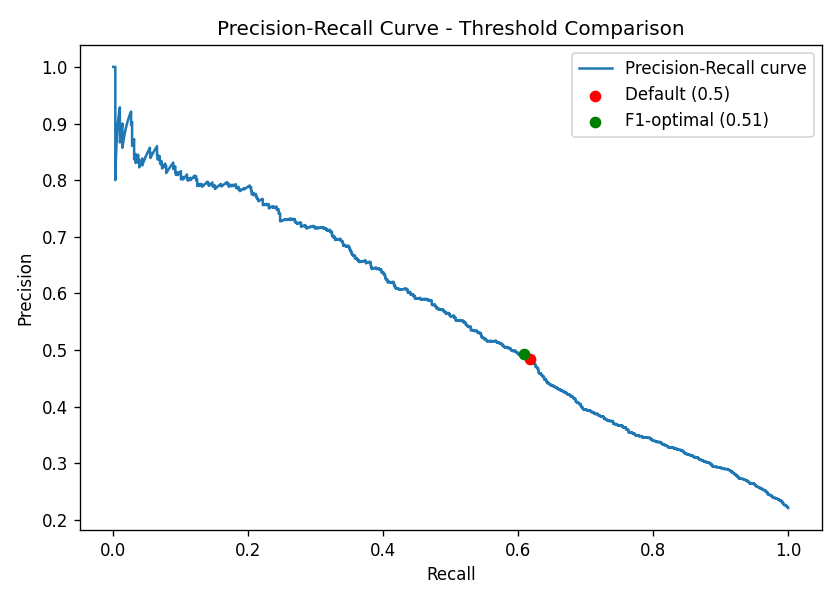
\includegraphics[width=0.75\textwidth]{plots/precision_recall_curve.png}
\caption{Precision-recall curve with the default (0.5) and F1-optimal
(0.5109) thresholds marked.}
\label{fig:pr_curve}
\end{figure}

The F1-optimal threshold was found to be \textbf{0.5109} -- barely
different from the naive 0.5 default. This is itself a meaningful finding:
it indicates the model's predicted probabilities were already reasonably
well-calibrated for this decision boundary, rather than systematically
skewed. At this threshold, F1 improved marginally to \textbf{0.545}.

A second, recall-favoring threshold (0.345, with a precision floor of
0.35) was also computed, achieving 77.3\% recall. This is documented as a
concrete alternative for a deployment context where missing an actual
defaulter (a false negative) is judged costlier than a false alarm --
though the specific floor of 0.35 was chosen illustratively here, and a
real deployment would derive it from an actual cost-of-error analysis
rather than a fixed convention.

\begin{table}[H]
\centering
\caption{Final model summary across candidate thresholds.}
\label{tab:final}
\begin{tabular}{lcccc}
\toprule
\textbf{Threshold} & \textbf{Precision} & \textbf{Recall} & \textbf{F1} & \textbf{AUC} \\
\midrule
0.500 (default)              & 0.4835 & 0.6172 & 0.5422 & 0.7781 \\
\textbf{0.5109 (F1-optimal, deployed)} & -- & -- & \textbf{0.5447} & \textbf{0.7781} \\
0.345 (recall-favoring)      & $\geq$0.35 & 0.7732 & -- & 0.7781 \\
\bottomrule
\end{tabular}
\end{table}

\subsection{Explainability}
SHAP (SHapley Additive exPlanations)~\cite{shap} values were computed on a
1{,}000-row sample of the test set using \texttt{TreeExplainer}, to
understand which features drive the model's predictions
(Figure~\ref{fig:shap}).

\begin{figure}[H]
\centering
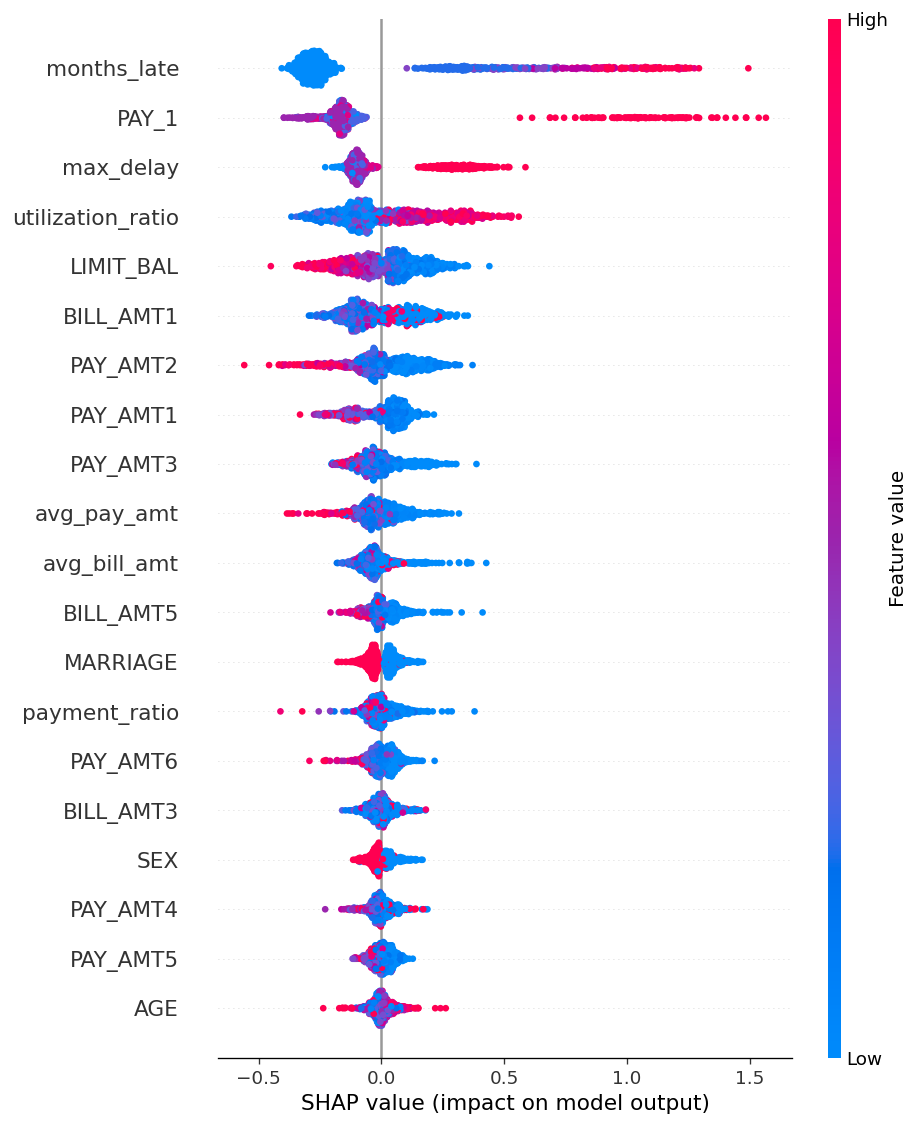
\includegraphics[width=0.75\textwidth]{plots/shap_summary.png}
\caption{SHAP summary plot showing feature impact on model output.}
\label{fig:shap}
\end{figure}

\begin{table}[H]
\centering
\caption{Top 5 features by mean absolute SHAP value.}
\label{tab:shap}
\begin{tabular}{lc}
\toprule
\textbf{Feature} & \textbf{Mean |SHAP value|} \\
\midrule
months\_late       & 0.3946 \\
PAY\_1             & 0.2655 \\
max\_delay         & 0.1615 \\
utilization\_ratio & 0.1541 \\
LIMIT\_BAL         & 0.1172 \\
\bottomrule
\end{tabular}
\end{table}

The two most important features -- \texttt{months\_late} and
\texttt{PAY\_1} (most recent repayment status) -- both relate directly to
recent repayment behavior. This aligns with financial domain intuition
(recent behavior is predictive of near-future behavior) and provides
evidence that the model has learned a plausible, explainable signal
rather than an artifact of the data.

% ============================================================
\section{System Architecture}
% ============================================================

Beyond the model itself, the system was built as a multi-component
service, illustrated in Figure~\ref{fig:architecture}.

\begin{figure}[H]
\centering
\begin{verbatim}
                    Frontend (HTML/JS/Tailwind) -- Vercel
                                |
                        HTTPS (CORS-enabled)
                                |
                     FastAPI backend -- Render
                    /predict  /batch-predict  /model/info
                       |                  |
                PostgreSQL          Redis (cache + queue)
                (predictions,              |
                 model_versions)      RQ Worker
                                  (async batch scoring)
\end{verbatim}
\caption{System architecture: frontend, API, persistence, and
asynchronous processing layers.}
\label{fig:architecture}
\end{figure}

\subsection{API layer}
A FastAPI backend exposes the model through validated, typed endpoints
(Pydantic schemas enforce the exact 23-column input schema before any
data reaches the model). Endpoints include synchronous single prediction
(\texttt{/predict}), asynchronous batch prediction
(\texttt{/batch-predict}), model metadata (\texttt{/model/info}), and
prediction lookup by ID (\texttt{/predictions/\{id\}}).

The same \texttt{src/} preprocessing and inference modules are shared
between the API, the notebooks, and the background worker -- this was a
deliberate design choice to eliminate ``training/serving skew,'' a common
real-world failure mode where the code path used to train a model
silently diverges from the code path used to serve it.

\subsection{Persistence and caching}
Every prediction is persisted to PostgreSQL (input data, prediction,
probability, and a foreign key to the model version that produced it),
enabling auditability and lookup. Redis caches predictions by a
deterministic hash of the input payload (order-independent), with a
5-minute TTL, to avoid redundant computation on repeated identical
requests. Both the database and cache layers are designed to fail
gracefully: if either is unreachable, the API still returns a correct
prediction, simply without persistence or caching for that request. This
was verified directly by running the API with no database or cache
available and confirming predictions still succeeded.

\subsection{Asynchronous batch processing}
Large batch scoring requests (CSV uploads) are handled asynchronously
using RQ (Redis Queue): the API enqueues the job and returns a job ID
immediately, rather than blocking the HTTP connection for the duration of
scoring. A separate worker process consumes the queue, scores the batch
using the identical pipeline as single predictions, and persists results,
which can then be polled via a status endpoint.

\subsubsection{A cross-platform bug and its resolution}
During development, RQ's default \texttt{Worker} class was found to crash
immediately on Windows with \texttt{AttributeError: module `os' has no
attribute `fork'}. This is because RQ's default worker isolates each job
in a forked child process using the POSIX \texttt{os.fork()} system call,
which does not exist on Windows. This was resolved by detecting the
platform at runtime and substituting RQ's \texttt{SimpleWorker} (which
executes jobs in-process, without forking) on Windows, while retaining the
standard process-forking \texttt{Worker} on Unix-like systems -- preserving
full process isolation in the Linux-based Docker deployment while
remaining developer-friendly on Windows.

\subsection{Containerization}
The full stack (API, worker, PostgreSQL, Redis) is defined in a single
\texttt{docker-compose.yml}, allowing the entire system to be started
with one command (\texttt{docker compose up --build}). Both the API and
worker share a single \texttt{Dockerfile} and Python environment, differing
only in their startup command, to avoid maintaining duplicate, divergent
container definitions. Exact model-training library versions
(\texttt{scikit-learn==1.8.0}, \texttt{lightgbm==4.7.0}) are pinned in
\texttt{requirements.txt} to eliminate a version-mismatch warning observed
when a newer scikit-learn attempted to unpickle a model trained on an
older version -- a subtle reproducibility issue that is easy to overlook.

\subsection{Deployment and a free-tier constraint}
The backend is deployed on Render and the static frontend on Vercel,
communicating over HTTPS with CORS explicitly enabled. One notable
constraint surfaced during deployment: Render's free tier does not offer
a standalone ``background worker'' service type (a paid-plan feature),
which the originally designed architecture required. Rather than
abandoning asynchronous processing or paying for a second service, the
worker was instead launched as a genuine separate OS subprocess from
within the API service's startup routine. This is explicitly documented
in the codebase as a free-tier trade-off, distinct from the architecturally
``correct'' setup (separate containers) that Docker Compose runs locally --
an example of adapting a design to real infrastructure constraints while
being transparent about the compromise made.

% ============================================================
\section{Results Summary}
% ============================================================

\begin{table}[H]
\centering
\caption{End-to-end summary of modeling progress across iterations.}
\label{tab:summary}
\begin{tabular}{lcccc}
\toprule
\textbf{Stage} & \textbf{Precision} & \textbf{Recall} & \textbf{F1} & \textbf{AUC} \\
\midrule
Logistic Regression (baseline)     & 0.443 & 0.602 & 0.510 & 0.745 \\
LightGBM (baseline)                & 0.463 & 0.621 & 0.530 & 0.778 \\
LightGBM + SMOTE (rejected)        & 0.601 & 0.429 & 0.500 & 0.770 \\
LightGBM (tuned, 0.5 threshold)    & 0.484 & 0.617 & 0.542 & 0.778 \\
\textbf{LightGBM (tuned, final threshold)} & \textbf{--} & \textbf{--} & \textbf{0.545} & \textbf{0.778} \\
\bottomrule
\end{tabular}
\end{table}

The final deployed model represents a 6.8\% relative F1 improvement over
the initial LightGBM baseline (0.530 $\rightarrow$ 0.545), achieved
through evidence-based iteration: testing and rejecting SMOTE, tuning
hyperparameters against the correct metric, and calibrating the decision
threshold -- rather than a single modeling pass.

% ============================================================
\section{Discussion and Limitations}
% ============================================================

\subsection{On the performance ceiling}
This dataset is a well-known, difficult benchmark in the credit-scoring
literature. Published results using classical models (Logistic Regression,
Random Forest, SVM) on this same dataset typically report AUC in the
0.75--0.82 range and F1 scores well below 0.60, regardless of the
sophistication of preprocessing applied~\cite{yeh2009}. The results in this
report (AUC 0.778, F1 0.545) are consistent with this known ceiling. A
system reporting substantially higher numbers on this specific dataset
would warrant scrutiny for data leakage rather than celebration.

\subsection{Generalizability}
The model is trained on a single snapshot of Taiwanese consumer credit
data from 2005. Applying it to a different population, time period, or
currency/economic context without retraining would be inappropriate --
this is stated plainly in the project's README and is not a caveat
intended to be glossed over.

\subsection{Engineering trade-offs documented in this work}
Several trade-offs were made explicitly and documented rather than hidden:
\begin{itemize}[nosep]
    \item SMOTE was tested and rejected based on measured F1 degradation,
    not assumed to help by default.
    \item The Windows/Unix worker incompatibility was fixed with a
    platform-conditional implementation, preserving full process isolation
    where the platform allows it.
    \item The free-tier deployment constraint (no dedicated worker service)
    was worked around with a subprocess-based approach, explicitly
    distinguished in the codebase from the "correct" containerized
    architecture used locally.
\end{itemize}

\subsection{Future work}
\begin{itemize}[nosep]
    \item A real cost-sensitive threshold (rather than the illustrative
    0.35 precision floor used for the recall-favoring alternative), derived
    from an actual cost matrix if such a system were deployed commercially.
    \item Model monitoring for data drift on incoming batch predictions.
    \item CI/CD via GitHub Actions to run the test suite automatically on
    every push.
    \item A paid-tier deployment to eliminate free-tier cold-start latency
    and restore a fully separate worker service.
\end{itemize}

% ============================================================
\section{Conclusion}
% ============================================================

This project demonstrates a complete, evidence-driven machine learning
system: from raw, imperfect data through leakage-safe preprocessing,
honestly-evaluated imbalanced classification, measured (not assumed)
technique selection, explainability analysis, and a fully deployed,
containerized, multi-service production architecture. Every metric
reported in this document was independently verified against the
project's own generated artifacts (\texttt{model\_card.md},
\texttt{metrics.json}) rather than asserted, and every architectural
decision -- including the ones driven by real constraints such as a
Windows-specific bug and a free-tier hosting limitation -- is documented
alongside its reasoning. The live system is available at
\url{https://credit-risk-modeling.vercel.app}, with full source code at
\url{https://github.com/Saumi18/Credit-Risk-Modeling}.

% ============================================================
\begin{thebibliography}{9}

\bibitem{uci_dataset}
Yeh, I-Cheng. (2009). Default of Credit Card Clients. UCI Machine Learning
Repository. \url{https://archive.ics.uci.edu/dataset/350/default+of+credit+card+clients}

\bibitem{yeh2009}
Yeh, I-Cheng, and Che-hui Lien. ``The comparisons of data mining techniques
for the predictive accuracy of probability of default of credit card
clients.'' Expert Systems with Applications 36.2 (2009): 2473-2480.

\bibitem{optuna}
Akiba, T., Sano, S., Yanase, T., Ohta, T., \& Koyama, M. (2019). Optuna: A
Next-generation Hyperparameter Optimization Framework. KDD.

\bibitem{shap}
Lundberg, S. M., \& Lee, S. I. (2017). A Unified Approach to Interpreting
Model Predictions. NeurIPS.

\end{thebibliography}

\end{document}
